
% \section{Background} 
% \subsection{Subsection 1}
% \lipsum[10]
% \begin{enumerate}
%     \item Point 1
%     \item Point 2
%     \item Point 3
% \end{enumerate}
% \lipsum[1]

\section{Background}

In this section, we provide a technical background in WebAssembly, which is one of the key components of our solution. This technology appeared as consequence of the rapid evolution of software development, which introduced microservices as a dominant architectural paradigm, offering modularity, scalability, and improved resource optimization. Modern frameworks and technologies have emerged to address the challenges of orchestrating microservices effectively, including communication, performance tuning, and seamless deployment. Among these, WebAssembly (Wasm) has gained prominence as a portable and efficient runtime that bridges the gap between cloud and edge environments. This section explores notable microservice frameworks, the capabilities of WebAssembly, and its role as a unifying layer across diverse infrastructures.

\subsection{Microservice Frameworks}
Modern microservice frameworks, such as Service Weaver\cite{ghemawat2023towards} and Blueprint\cite{anand2023blueprint} simplify the challenges of microservice orchestration, such as communication, performance optimization, and reconfiguration.

Microservice frameworks provide a structured and organized approach to building, deploying, and managing microservices. These frameworks simplify the complex processes associated with microservice architecture, enabling developers to focus more on business logic rather than the intricacies of infrastructure. 

This decomposition allows optimization of existing resources, such as colocation of business logic modules. We take this into consideration when choosing our technology stack, the WebAssembly Stack, which standardizes decomposition with the WebAssembly Component Model.

Below, we discuss the two notable frameworks, Blueprint\cite{anand2023blueprint} and Service Weaver\cite{ghemawat2023towards}, which offer distinct features but present the same principal drawback.

\subsubsection{Blueprint Framework}
Blueprint\cite{anand2023blueprint} proposes a solution that simplifies microservice deployment by providing a toolchain to automatically build and deploy microservices. The framework generates code based on two key specifications:

\begin{itemize}
    \item \textbf{Workflow Specifications}: Defines the business logic of the application, which can be seen in Figure \ref{fig:workflow-spec}.
    \item \textbf{Wiring Specifications}: Details the scaffolding, including component interactions, logging, and RPC library integration. This code can be seen in figure \ref{fig:wiring-spec}
\end{itemize}

\begin{figure}[h!]
\centering
\begin{minipage}{0.48\textwidth}
    \centering
    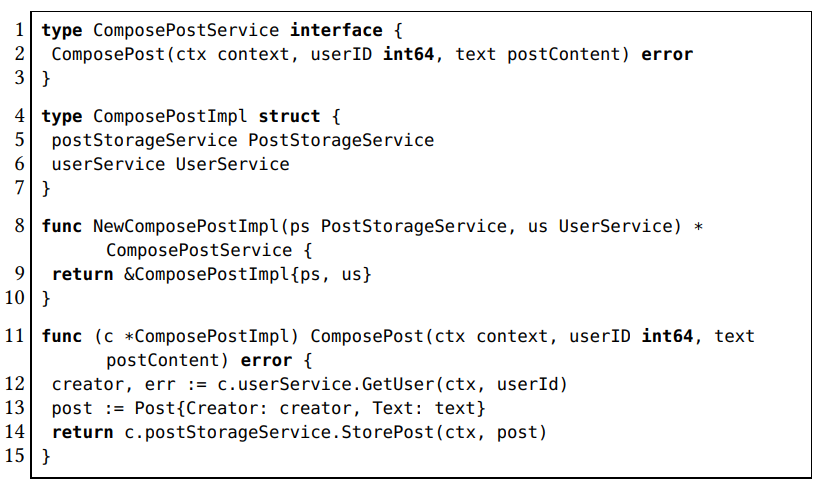
\includegraphics[width=\textwidth]{Images/workflow_spec.png}
    \caption{Workflow specification for defining business logic.}
    \label{fig:workflow-spec}
\end{minipage}
\hfill
\begin{minipage}{0.48\textwidth}
    \centering
    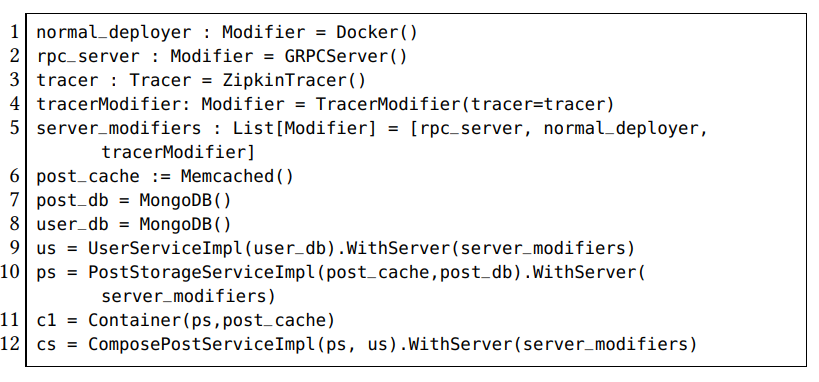
\includegraphics[width=\textwidth]{Images/wiring_spec.png}
    \caption{Wiring specification detailing the microservices scaffolding.}
    \label{fig:wiring-spec}
\end{minipage}
\end{figure}

This architecture allows for easier reconfiguration; for instance, switching between RPC libraries or adding logging typically requires only 1-5 lines of changes in the wiring specifications.

While Blueprint significantly reduces the complexity of microservice management, it is not entirely seamless and mandates developers to work within its framework.

\subsubsection{Service Weaver Framework}
Service Weaver\cite{ghemawat2023towards} addresses five challenges of microservices: performance degradation, correctness issues, management complexity, API versioning constraints, and slowed application development. To resolve these issues, Service Weaver introduces a framework that enables:

\begin{itemize}
    \item \textbf{Service Co-location}: Enables function calls to operate locally, or as remote RPCs based on runtime decisions.
    \item \textbf{Simplified Microservice Testing}: Integration testing is simplified, because local modes can function effectively as unit tests without requiring remote calls.
    \item \textbf{API Versioning}: Mitigates API versioning problems due to updates to the application code being applied holistically.
\end{itemize}

While having multiple advantages, Service Weaver \cite{ghemawat2023towards} also requires developers to adopt its specific framework, limiting developer experience.

\subsection{WebAssembly (Wasm)}
WebAssembly (Wasm) is a portable, low-level binary instruction format designed to serve as a compilation target for various programming languages, such as C, C++, and Rust. Initially created for the web, Wasm has become a transformative technology that now spans across domains like cloud computing, edge computing, IoT, and even serverless architectures.

Wasm allows developers to write applications in their preferred languages and compile them into an intermediate format that is both efficient and portable. Its architecture provides near-native execution speed while maintaining strong security guarantees, making it ideal for performance-critical applications.

Key advantages of Wasm include:
\begin{itemize}
\item \textbf{Portability}: Wasm binaries can run on any platform equipped with a browser or other runtime that supports Wasm.
\item \textbf{Efficiency}: Wasm provides low-latency execution with fast startup times, useful for cloud and edge workloads.
\item \textbf{Isolation}: Applications run securely within a sandboxed environment, reducing risks of unauthorized access or corruption.
\end{itemize}

In addition to its primary role in web applications, Wasm is increasingly being adopted in edge computing scenarios, where its efficiency and portability allow developers to deploy lightweight containers on low-resource devices.

\subsection{WebAssembly System Interface (WASI)}
The WebAssembly System Interface (WASI) extends WebAssembly's capabilities beyond the browser, enabling interaction with system resources. It provides a set of APIs for operating system functionalities, such as file I/O, network sockets, clocks, and process management.

WASI ensures that Wasm modules can run across different platforms, from edge devices to large cloud servers, without requiring changes to the application code.

Currently, WASI is available in two versions:
\begin{itemize}
\item \textbf{WASI v1}: A foundational system interface supporting essential features like file access and most system calls.
\item \textbf{WASI v2}: Introduces a component model that enables modular, reusable, and interoperable WebAssembly components. This model facilitates better integration between different programming languages and tools with a common interface (WIT).
\end{itemize}

\subsection{The Component Model}
The Component Model, introduced in WASI v2, is a significant advancement in WebAssembly's modular ecosystem. It provides a higher-level abstraction for Wasm modules, allowing dynamic linking and safe interaction between components.

With a \textbf{shared-nothing} architecture, components interact through explicit interfaces. This ensures strong isolation while enabling clean communication. Key features of the Component Model include:
\begin{itemize}
\item \textbf{Dynamic Linking}: Unlike WASI v1 which does not support \textbf{dlopen} nor \textbf{dlsym} (which are explained in Section \ref{sec-3.1}), modules inside a component can be loaded at runtime.
\item \textbf{Interoperability}: Components written in different languages communicate via standardized WIT interfaces.
\item \textbf{Memory Encapsulation}: Each module manages its linear memory, ensuring no unintended sharing of resources.
\end{itemize}

\subsection{WebAssembly Interface Types (WIT)}
The WebAssembly Interface Types (WIT) specification simplifies interoperability between modules written in different programming languages. Traditionally, WebAssembly modules used low-level types like integers and pointers, which made sharing complex data structures across modules difficult.

WIT introduces high-level types such as strings, lists, and records, allowing modules to communicate seamlessly. It serves as a bridge, enabling components written in Rust, Go, or C++ to interact without needing extensive type conversions or manual serialization.

Key contributions of WIT include:
\begin{itemize}
\item \textbf{Simplified Communication}: Abstracts low-level complexities to enable clear and structured module interactions.
\item \textbf{Immutable Interface}: Due to the immutable interface, which is enforced by the component model's shared nothing architecture, where each component has its own linear memory, components may be distributed.
\item \textbf{Language Agnosticism}: Promotes modular development across multiple programming languages with shared types.
\item \textbf{Type Safety}: Reduces errors by ensuring consistency in data representation.
\end{itemize}

\subsection{WebAssembly RPC (wRPC)}
WebAssembly RPC (wRPC) is a protocol that facilitates Remote Procedure Calls (RPC) between Wasm modules. By using Wasm's component model architecture, wRPC enables distributed communication across environments, such as edge servers and cloud infrastructure.

This approach abstracts the complexities of component interaction and allows function calls between remote Wasm components to appear as local operations. wRPC enhances scalability by enabling distributed execution while preserving Wasm's strong isolation guarantees.

The \textbf{wRPC protocol} is a transport-agnostic system designed for asynchronous communication of WebAssembly Interface Types (WIT) function calls within a client-server architecture. Supporting multiplexed, bidirectional data streams, it utilizes the component model value definition encoding for serialization.

\subsubsection*{Key Features}
\begin{itemize}
\item \textbf{Transport Protocols}: Compatible with TCP, QUIC, Unix Domain Sockets, and NATS.io, among others.
\item \textbf{Multiplexing}: Supports concurrent handling of multiple data streams, enabling efficient execution of asynchronous functions such as input/output streams.
\item \textbf{Encoding}: Implements the component model's value encoding, extended for streams ($list$).
\end{itemize}

\subsubsection*{Framing Specification}
Messages in wRPC start with a version byte and a \texttt{header} structure, followed by frames containing indexed paths and data payloads, which:

\begin{itemize}
\item Facilitates resource-efficient RPC calls.
\item Offers modularity across various transport mechanisms.
\item Seamlessly integrates with WebAssembly's component model.
\end{itemize}

This makes wRPC a good choice for high-performance distributed systems and WebAssembly applications requiring remote module execution such as our work.

\subsection{WebAssembly as a common layer across the cloud-edge continuum}

The use of WebAssembly as a common layer across the cloud-edge continuum has been explored by
Ménétrey et al \cite{menetrey2022webassembly}, who highlight how WebAssembly can bridge the gap between proprietary silos across
cloud, edge, and IoT devices, while maintaining strong performance. 

To verify that WebAssembly is
able to achieve strong performance compared to native and across the cloud-edge continuum, they run
benchmarks on a x86 intel cloud server and an arm edge processor. These benchmarks consist of
the PolyBench/C Benchmarks and benchmarking a WebAssembly compiled version of SQLLite.
These show that the slowdown relative to the native version varied from 1.3X on the PolyBench/C Benchmarks
and at maximum 2.7x in the x86 processor, the performance also has improved over time, with previous
versions of the WAMR runtime they used in 2020 having considerable worse performance (4.1x slowdown
compared to the native architecture). 

They also show that security guarantees of the execution of the applications can be achieved despite running these applications on untrusted edge hardware, by using
Trusted Execution Environments (TEEs), such as Intel SGX and Arm TrustZone.

% Consider Table~\ref{tab:example} below.
%% For tables, see:
% - https://jdhao.github.io/2019/08/27/latex_table_with_booktabs/
% - https://people.inf.ethz.ch/markusp/teaching/guides/guide-tables.pdf
% \begin{table}
%     \centering
%     \caption{Description}
%     \label{tab:example}
%     \begin{tabular}{@{}lllll@{}}
%         \toprule
%         \multirow{2}{*}[-1em]{Models} & \multicolumn{3}{c}{Metric 1} & Metric 2\\
%         \addlinespace[10pt]
%         \cmidrule(lr){2-4} \cmidrule(lr){5-5} \\
%         {} & precision & recall & F-score  & R@10 \\
%         \midrule
%         model 1 & 0.67  & 0.8 & 0.729  & 0.75 \\
%         model 2 & 0.8 & 0.9 & 0.847 & 0.85 \\
%         \bottomrule
%     \end{tabular}
% \end{table}

